\section{Proteção da \acrshort{api} de dados}

Para proteger as rotas da \acrshort{api} é necessário haver métodos de verificação dos \textit{tokens} com o objetivo de decidir se o utilizador/Chave \acrshort{api} pode aceder a uma determinada rota. De seguida será apresentado o pseudo-código de verificação dos \textit{tokens} tendo em conta que os utilizadores registados conseguem aceder a todas as rotas que as Chaves \acrshort{api} conseguem mas que o inverso não acontece. Ou seja, um utilizador registado até o de nível mais baixo por exemplo, consegue aceder a todas as rotas que as Chaves \acrshort{api} tem acesso e mais algumas nas quais as Chaves \acrshort{api} não têm permissões de acesso.

Após se identificar o \textit{token}, verifica-se o \textit{token}. Esta verificação varia de acordo se o \textit{token} é de um utilizador ou de uma Chave \acrshort{api}. Caso seja de uma chave \acrshort{api}, verifica-se se existe a entrada no \textit{MongoDB} e se a chave \acrshort{api} ainda se encontra ativa. Em caso afirmativo, procede-se para a verificação do \textit{token} (se ainda não expirou) com recurso ao segredo. No caso de um utilizador verifica-se se o \textit{token} ainda não expirou e se a operação tiver restrições quanto ao nível de utilizador que pode aceder, verifica-se também se o nível presente no \textit{token} permite realizar a operação.

Por forma a validar se uma Chave \acrshort{api} pode aceder a uma determinada rota pode ser executada a seguinte função em \textit{middleware}:
\begin{lstlisting}[language=pseudocode, caption=Verificação se um pedido com uma determinada Chave \acrshort{api} pode ser efetuado]
function isLoggedInKey(req, res, next)
    key = getJWTfromHeaderOrQueryString('apikey')

    if key then
        keyBD = getKeyFromMongoDB(key)
        if keyBD then
            res = jwt.verify(key, secretForAPIkey)
            if res != expired then
                if keyBD.active == True then
                    return next()
                else
                    return err
            else
                return err
        else
            return err
    else
        return isLoggedInUser(req, res, next)
\end{lstlisting}
É importante destacar a chamada da função \texttt{isLoggedInUser} que é executada no caso de não ser detetado uma Chave \acrshort{api} no pedido (na \textit{header} \textit{Authorization} ou na \textit{query string} \texttt{apikey}) e como tal, com essa chamada, tenta-se perceber se afinal foi passado um \textit{token} de um utilizador já que todos os utilizadores conseguem aceder às rotas que as Chaves \acrshort{api} conseguem como já referido.

No seguimento, para validar se um determinado \textit{token} de um utilizador registado pode aceder a uma determinada rota é executada a seguinte função em \textit{middleware}:
\begin{lstlisting}[language=pseudocode, caption=Verificação se um pedido com um determinado \textit{token} de um utilizador registado pode ser efetuado]
JWTstrategy = passport-jwt.Strategy

passport.use("jwt", new JWTstrategy(
    secretOrKey: secret,
    algorithms: ["HS256"],
    jwtFromRequest: getJWTfromHeaderOrQueryString('token')
, (token, done) => done(null, token)))

function isLoggedInUser(req, res, next)
    passport.authenticate("jwt", { session: false }, function (err, user, info)
        if err then
            return err
        if !user then
            return err
        req.logIn(user, function(err)
            if err then
                return err

            next()
        )
    )(req, res, next)
\end{lstlisting}

Os \textit{tokens} tanto das Chaves \acrshort{api} como de \textit{tokens} de utilizadores registados são obtidos através da utilização de extratores presentes na estratégia \texttt{passport-jwt} do \texttt{passport}. Assim para extrair o \textit{token} da \textit{query string} basta:
\begin{lstlisting}[language=javascript, caption=Extração do \textit{token} da \textit{query string}]
var ExtractJWT = require("passport-jwt").ExtractJwt
token = ExtractJWT.fromUrlQueryParameter("<nome do campo, 'token' ou 'apikey' no caso da CLAV>")
\end{lstlisting}
Já para extrair o \textit{token} da \textit{header} \textit{Authorization} basta:
\begin{lstlisting}[language=javascript, caption=Extração do \textit{token} da \textit{heaer} \textit{Authorization}]
var ExtractJWT = require("passport-jwt").ExtractJwt
token = ExtractJWT.fromAuthHeaderWithScheme("<palavra antes do token, 'Bearer' no caso dum bearer token, 'token' ou 'apikey' no caso da CLAV>")
\end{lstlisting}

Para verificar se o utilizador registado tem um nível suficiente para aceder a uma rota, depois de se verificar que o utilizador está autenticado (\texttt{isLoggedInUser}), deve-se executar também em \textit{middleware} a seguinte função:
\begin{lstlisting}[language=pseudocode, caption=Verificação se um utilizador registado tem permissões suficientes para aceder a uma determinada rota]
function checkLevel(clearance)
    return function(req, res, next)
        havePermissions = False

        if clearance is Array then
            if req.user.level in clearance then
                havePermissions = True
        else
            if req.user.level >= clearance then
                havePermissions = True

        if havePermissions then
            return next()
        else
            return err
\end{lstlisting}
Ou seja, a variável \texttt{clearance} poderá ser uma lista de números ou apenas um número. No primeiro caso verifica-se que o nível do utilizador está presente na lista, em caso afirmativo então o utilizador tem permissões para aceder. Já no segundo caso, o utilizador só terá permissões para aceder se o seu nível foi igual ou superior ao \texttt{clearance}.

Com estas três funções (\texttt{isLoggedInKey}, \texttt{isLoggedInUser} e \texttt{checkLevel}) é possível proceder à proteção da \acrshort{api} da \acrshort{clav} garantindo que utilizadores com diferentes níveis de acesso apenas conseguem aceder ao que lhes é permitido.

%TODO
TODO: completar

\section{Autenticação através de \acrshort{cmd}}
%TODO
TODO

\section{Documentação da \acrshort{api} da \acrshort{clav}}
%TODO
TODO: Apresentar imagens do swagger UI

\section{Exportação de dados}
Um dos requisitos da \acrshort{api} da \acrshort{clav} é permitir a exportação de Classes, Entidades, Tipologias e Legislações em formato \acrshort{json}, \acrshort{xml} e \acrshort{csv}. Deve também permitir exportar toda a ontologia do projeto nos formatos \acrshort{turtle}, \acrshort{json-ld} e \acrshort{rdf}/\acrshort{xml}.

Para a primeira parte foi necessário desenvolver dois conversores, de \acrshort{json} para \acrshort{xml} e de \acrshort{json} para \acrshort{csv} visto que o \acrshort{json} já é por predefinição devolvido.

\subsection{\acrshort{xml}}
O conversor de \acrshort{json} para \acrshort{xml} criado é representado pelo algoritmo presente no anexo~\ref{exem:convXML}.

Apresenta-se no anexo~\ref{conv:jsonTOxml} uma conversão exemplo.

\subsection{\acrshort{csv}}

Da mesma forma que o \acrshort{xml}, o \acrshort{csv} é convertido sem recurso a uma biblioteca que converta já de si o \acrshort{json} para \acrshort{csv} visto que cada objeto \acrshort{json} a exportar necessita de uma exportação personalizada para \acrshort{csv}. Ao contrário do conversor desenvolvido para \acrshort{xml}, o conversor para \acrshort{csv} não converte qualquer objeto para \acrshort{csv} mas apenas um conjunto restrito de objetos \acrshort{json}.

O algoritmo de conversão de \acrshort{json} para \acrshort{csv} desenvolvido pode ser visualizado no anexo~\ref{exem:convCSV}.

O conjunto de objetos permitidos é lista de classes, de entidades, de tipologias e de legislações e objeto de classe, de entidade, de tipologia e de legislação.

Quanto à conversão em si, possui uma estrutura interna durante a conversão. Esta estrutura é uma lista de listas, em que cada lista representa uma linha do \acrshort{csv}. Cada elemento de uma das listas representará uma célula do \acrshort{csv}. A primeira lista será a primeira linha do \acrshort{csv} e como tal possuirá os títulos. As restantes listas serão as linhas seguintes do \acrshort{csv} em que cada elemento possuirá os valores já transformados em \textit{strings} dos campos dos objetos.

Para além desta estrutura interna existe um dicionário que permite agilizar o algoritmo de conversão. Este dicionário possuirá vários dicionários, um por cada objeto (Classe, Entidade, Tipologia e Legislação) em que cada um destes dicionários irá ter como chaves os campos a converter. Para cada um destes campos existe um tuplo em que na primeira posição está presente o título a colocar no \acrshort{csv} referente a este campo e na segunda posição a função de transformação a executar para o valor do campo. Há a presença de três casos especiais:
\begin{itemize}
    \item Quando o valor do campo é uma lista de objetos e pretendemos apenas um dos campos de cada objeto, o valor do campo deve ser \verb|campo_campoDoObjeto| e deve ser usada a função de transformação \verb|map_value(<campoDoObjeto>)|
    \item Quando o valor do campo é um objeto do qual irá resultar vários títulos, na primeira posição do tuplo deve estar presente uma \textit{string} vazia e a função de transformação deve devolver uma lista com duas posições, na primeira com os títulos e na segunda com os valores transformados dos campos
    \item Quando o valor do campo é uma lista de objetos Classe, Entidade, Tipologia ou Legislação a primeira posição do tuplo deve ser \texttt{null} e a função de transformação deve devolver uma lista de listas sem a primeira linha de títulos
\end{itemize}
No caso da conversão de um objeto e consoante a transformação (ou seja, o título do dicionário) a inserção realizada na lista de listas varia:
\begin{itemize}
    \item \verb|título == null|: concatena-se a lista de listas devolvida pela função de transformação à lista de listas
    \item \verb|título == ""|: concatena-se a lista dos elementos da primeira linha devolvida pela função de transformação com os elementos da primeira linha e realiza-se o mesmo para o caso da segunda linha devolvida, concatena-se a segunda linha com a segunda linha
    \item Nos restantes casos protege-se\footnote{colocar valor entre aspas (\texttt{"})} o título presente no dicionário e adiciona-se à primeira lista; para além disso, o valor transformado devolvido pela função de transformação é adicionado já protegido à segunda lista.
\end{itemize}

No caso da conversão de uma lista de objetos, para cada objeto será feita a conversão já apresentada para um objeto, onde depois é ignorada a linha dos títulos em todos os objetos exceto no primeiro objeto da lista onde é mantido os títulos gerados. Ou seja, na primeira linha estará presente os títulos e nas seguintes linhas, em cada linha estará presente os valores de um objeto.

O último passo seja para uma lista ou para um único objeto é transformar a estrutura interna no \acrshort{csv}. Este papel é desempenhado pela função \texttt{joinLines} em que os elementos de cada lista da lista são juntos de acordo com um separador (neste caso é usado o ponto e vírgula, ``\texttt{;}'') tornando a lista de listas numa lista de \textit{strings}. Por fim, as \textit{strings} desta lista são juntas através da inserção de novas linhas (``\texttt{\textbackslash{}n}'') entre cada \textit{string} gerando o \acrshort{csv} final.

No anexo~\ref{conv:jsonTOcsv} apresenta-se um exemplo de uma conversão, onde o ficheiro \acrshort{json} a converter é o mesmo usado para exemplificar a conversão de \acrshort{xml} presente em~\ref{exem:json}.

\subsection{Exportação da Ontologia}

%TODO: o que colocar?
TODO

\subsection{Exportação na \acrshort{api} de dados}

%TODO: explicar como foi colocado esta parte na API, como middleware
TODO

\subsection{Interface de Exportação}

%TODO: apresentar e falar da interface de exportação
TODO: apresentar e falar da interface de exportação

\section{Migração de \acrshort{http} para \acrshort{https}}

A partir dos requisitos já enunciados em~\ref{sec:sol_httpsReq} foram criadas duas \textit{scripts} uma para correr antes de iniciar o \textit{Nginx} e outra para correr depois de o \textit{Nginx} iniciar.

A \textit{script} que corre antes de iniciar o \textit{Nginx} instala o \texttt{openssl}, gera o certificado autoassinado e \acrshort{dh} \textit{parameters} para permitir o \textit{boot} do \textit{Nginx}.

Já a \textit{script} que corre após o inicio do \textit{Nginx} realiza o \textit{download} do \texttt{acme.sh}, instala-o, obtém o primeiro certificado para o(s) domínio(s) com o \texttt{acme.sh}, instala o certificado com o \texttt{acme.sh}, gera \acrshort{dh} \textit{parameters} mais fortes e, por fim, reunicia o \textit{Nginx} para que o novo certificado e \acrshort{dh} \textit{parameters} tenham efeito, ou seja, sejam usados pelo \textit{Nginx}.

Quanto à configuração do \textit{Nginx} entre a da \acrshort{api} de dados e a da interface à poucas diferenças. Estas consistem em que na configuração \textit{Nginx} na \acrshort{api} de dados é encaminhado os pedidos para o servidor em \textit{Node.js} enquanto que na configuração \textit{Nginx} da interface há duas variantes:
\begin{itemize}
    \item Apenas serve os ficheiros estáticos da interface
    \item Serve os ficheiros estáticos da interface e reencaminha os pedidos para a \acrshort{api} de dados, aqueles em que o caminho começa em \texttt{/<versão\_api>/} ou é igual a \texttt{/clav.yaml}.
\end{itemize}

Quanto às configurações comuns estas serão apresentadas de seguida, explicando para que servem.

Para cumprir o requisito de redirecionamento dos pedidos de \acrshort{http} para \acrshort{https} é colocado o seguinte bloco de código na configuração:
\begin{lstlisting}
  server {
    listen $HTTP_PORT;
    server_name localhost;

    location /.well-known/acme-challenge/ {
      alias /var/www/html/.well-known/acme-challenge/;
    }

    location / {
      return 301 https://$host$request_uri;
    }
  }
\end{lstlisting}
Além disso,

%TODO
TODO
%explicar config do nginx

\section{\acrshort{api} Gateway}

Nesta secção irá ser abordada a configuração do \textit{Kong} além do desenvolvimento do Serviço de Auth adicional para a proteção da \acrshort{api} de dados.

\subsection{Serviço de \textit{Auth}}
Este serviço desenvolvido em \textit{Node.js} tem como principal papel a autenticação e autorização dos pedidos efetuados. Além disso, este serviço irá tratar de verificar e gerar \textit{tokens} (\acrshort{jwt}s). Assim, este serviço disponibiliza cinco rotas:
\begin{description}
    \item[POST /auth] Autenticar e Autorizar um pedido. Recebe no \textit{body} o verbo, o caminho, a \textit{query string} e os cabeçalhos do pedido a efetuar para a \acrshort{api} de dados. Como resposta devolve respostas com \textit{\acrshort{http} status} 200 (O pedido pode ser efetuado à \acrshort{api}. Devolve no \textit{body}  a informação contida no \textit{token} se este for enviado no pedido.), 401 (\textit{token} inválido ou pedido sem autenticação para aceder a rota), 403 (Pedido sem autorização para aceder a rota) ou 404 (A rota não existe).

        Para saber quem pode aceder determinada rota, o Serviço de \textit{Auth} possui um dicionário em que cada chave é um verbo \acrshort{http} e em cada verbo existe um dicionário com as vários caminhos desse verbo. A cada caminho é associado um valor que indica quem pode aceder a rota. Este valor é:
        \begin{itemize}
            \item \textbf{-1:} Todos podem aceder
            \item \textbf{0:} Só podem aceder Chaves API autenticadas ou utilizadores autenticados
            \item \textbf{Um número maior que 0:} Só podem aceder utilizadores autenticados com nível igual ou superior ao número
            \item \textbf{Lista de números maiores que 0:} Só podem aceder utilizadores autenticados com nível presente nesta lista
        \end{itemize}
        A ordem dos caminhos em cada verbo é importante visto que as rotas são testadas por ordem e, quando há um \textit{match}, é assumido que é essa a rota do pedido não sendo testado o resto dos caminhos.

        Consoante o valor obtido do dicionário é feita a autenticação e autorização necessária para a rota. Caso não seja obtido um valor, assume-se que a rota não existe na \acrshort{api} de dados.

        Sempre que for acrescentada uma nova rota na \acrshort{api} de dados é necessário adicionar essa neste dicionário com as devidas permissões.
    \item[POST /user/sign] Gerar um \textit{token} para um utilizador. Recebe no \textit{body} do pedido a informação do utilizador e o tempo de expiração a usar para o \textit{token}. Como resposta devolve o \textit{token} gerado.
    \item[POST /user/verify] Verificar um \textit{token} de um utilizador. Recebe no \textit{body} o \textit{token} do utilizador. Como resposta, caso o \textit{token} seja válido, devolve a informação contida no \textit{token}.
    \item[POST /apikey/sign] Gerar um \textit{token} para uma Chave API. Recebe no \textit{body} do pedido a informação da Chave API e o tempo de expiração a usar para o \textit{token}. Como resposta devolve o \textit{token} gerado.
    \item[POST /apikey/verify] Verificar um \textit{token} de uma Chave API. Recebe no \textit{body} o \textit{token} da Chave API. Como resposta, caso o \textit{token} seja válido, devolve a informação contida no \textit{token}.
\end{description}

A necessidade de rotas diferentes para utilizadores e Chaves API deve-se ao facto de serem usadas pares de chave pública/privada diferentes para gerar e verificar os \textit{tokens}. Para esta geração e verificação é usada a mesma biblioteca usada até agora, \textit{jsonwebtoken}. Continua-se também a usar os extratores da biblioteca \textit{passport-jwt} para obter os \textit{tokens} dos pedidos, mas já não se recorre ao \textit{passport} para proceder à autenticação visto não ser necessária.

Com a existência deste serviço, a \acrshort{api} de dados deixou de estar protegida e em casos que necessita de forma excecional a verificação ou a geração de \textit{tokens} recorre à \acrshort{api} do Serviço de \textit{Auth}. Apesar disso continua a ser essencial que a \acrshort{api} de dados saiba quem realizou o pedido. Essa informação será enviada num cabeçalho pelo \textit{Kong} algo que será explicado na próxima secção.

\subsection{\textit{Plugin} \texttt{external-auth}}
Como já referido anteriormente não é possível, usando os plugins disponíveis do \textit{Kong}, obter uma proteção semelhante à presente na \acrshort{api} de dados. Para resolver esta situação havia duas hipóteses, criar um plugin que trata da autenticação e da autorização ou criar um plugin que interceta os pedidos, realiza um pedido a um serviço externo para tratar da autenticação e da autorização, e consoante a resposta deixa ou não o pedido ser realizado. A segunda hipótese foi a escolhida visto que implica a criação de um plugin de menores dimensões, que tem de ser desenvolvido em \textit{Lua}, e permite por outro lado aproveitar parte do código de autenticação e autorização presente na \acrshort{api} de dados e usá-lo no serviço externo. Ou seja, é uma abordagem mais rápida e simples para além de que este \textit{plugin} de menores dimensões encontrava-se já em parte desenvolvido\footnote{Ver \url{https://github.com/aunkenlabs/kong-external-auth}} onde foi apenas necessário realizar algumas melhorias como a possibilidade de devolver respostas 403 e 404 entre outras alterações\footnote{Ver \url{https://github.com/jcm300/kong-external-auth}}.

De uma forma mais permenorizada, quando um pedido é recebido pelo \textit{Kong}, este pedido poderá passar por vários plugins de acordo com a configuração usada antes e após ser efetuado o pedido à \acrshort{api} de dados. O plugin \texttt{external-auth} se adicionado na configuração é executado antes do pedido ser efetuado à \acrshort{api} de dados. Este plugin obtém do pedido o caminho, verbo, \textit{query string} e cabeçalhos e envia-os no \textit{body} para o serviço externo. Quando o plugin recebe a resposta do serviço externo, consoante o \textit{\acrshort{http} status}:
\begin{itemize}
    \item 200: Insere no pedido a efetuar à \acrshort{api} de dados o cabeçalho \textit{CLAV-Auth} onde é enviado em formato \textit{string} a resposta do serviço externo
    \item 401: Devolve uma resposta de erro para o utilizador com \textit{\acrshort{http} status} 401
    \item 403: Devolve uma resposta de erro para o utilizador com \textit{\acrshort{http} status} 403
    \item 404: Devolve uma resposta de erro para o utilizador com \textit{\acrshort{http} status} 404
    \item Restantes: Devolve uma resposta de erro para o utilizador com \textit{\acrshort{http} status} 401

\end{itemize}

Portanto quando um pedido possui autenticação e autorização pelo serviço externo, este pedido inclui também um cabeçalho \textit{CLAV-Auth} onde estará presente a informação presente no \textit{token}, seja de um utilizador ou de uma Chave API. Este cabeçalho será interpretado pela \acrshort{api} de dados por forma a esta saber quem realizou o pedido. No caso do cabeçalho não ser enviado, for vazio ou num formato incorreto, a \acrshort{api} de dados irá considerar o pedido foi efetuado por alguém ``Desconhecido''.

\subsection{Configuração \textit{Kong}}
O \textit{Kong} pode ser configurado através de um ficheiro de configuração \texttt{.conf} onde é definido o modo em que executa, possíveis ligações a bases de dados, configurações do Nginx entre outros. Contudo não é neste ficheiro que se define o comportamento que o \textit{Kong} efetua quando recebe determinado pedido, apesar de se puder alterar algum comportamento através de configurações do Nginx. Para definir o comportamento do \textit{Kong} há três hipóteses. A que foi escolhida, configuração declarativa, permite que o \textit{Kong} execute sem necessitar de uma base de dados para armazenar as configurações visto que as configurações são definidas num ficheiro \acrshort{yaml} ou \acrshort{json} que é carregado para memória. Assim não se sobrecarrega desnecessariamente o servidor que executa o \textit{Kong}.

Para usar este configuração declarativa é necessário no ficheiro de configuração \texttt{.conf} colocar a diretiva \texttt{database} com o valor \texttt{off} e a diretiva \texttt{declarative\_config} com o caminho do ficheiro da configuração declarativa.

Na configuração declarativa são usados vários \textit{plugins} a maioria desenvolvidos pelo \textit{Kong} exceto o \textit{external-auth}. Por predefinição os plugins do \textit{Kong} estão disponíveis. Para se puder usar \textit{plugins} externos é necessário indicá-los no ficheiro \textit{.conf} na diretiva \texttt{plugins}. Assim o valor aqui colocado foi \texttt{blunded,external-auth} indicando que se pretende usar os plugins do \textit{Kong} (\texttt{blunded}) e o \textit{external-auth}. Antes de iniciar o \textit{Kong} será depois necessário instalar o \textit{plugin} \textit{external-auth}. No ficheiro \textit{.conf} é também indicado para onde os logs de erro e acesso são enviados sendo os de erro enviados para o \texttt{stderr} e os de acesso para o \texttt{stdout}. Além disso indicasse também em que portas (\acrshort{http} e \acrshort{https}) o \textit{Kong} irá receber os pedidos bem como em que portas está acessível a \acrshort{api} de administrador (como é usada uma configuração declarativa esta \acrshort{api} será apenas de leitura).

O primeiro passo na configuração declarativa foi adicionar o serviço da \acrshort{api} de dados e associar desde logo o \textit{plugin} necessário para a proteção da \acrshort{api} de dados:
\begin{lstlisting}[language=yaml, caption=Configuração declarativa do \textit{Kong}: \acrshort{api} de dados]
services:
  - name: API
    url: ${API_HOST}
    routes:
      - name: TodasRotas
        paths:
          - /
    plugins:
      - name: external-auth
        config:
          url: ${SERVER_AUTH_HOST}
          path: /auth
\end{lstlisting}
Com esta configuração inicial o \textit{Kong} reencaminha todos os pedidos que comecem por \texttt{/} para a \acrshort{api} de dados, usando neste serviço o \textit{plugin} \texttt{external-auth} já descrito. Temos assim uma primeira versão funcional com autenticação e autorização da \acrshort{api} de dados.

Contudo a \acrshort{api} de dados necessita de permitir \acrshort{cors} e para tal é adicionado o \textit{plugin} do \textit{Kong} chamado \texttt{cors}\cite{kongCORS}:
\begin{lstlisting}[language=yaml, caption=Configuração declarativa do \textit{Kong}: \textit{plugin} \texttt{cors}]
services:
  - name: API
    ...
    plugins:
      ...
      - name: cors
        service: API
        config:
          origins:
            - '*'
          methods:
            - GET
            ...
          headers:
            - Accept
            ...
          credentials: true
\end{lstlisting}
Além deste foram adicionados mais 3 \textit{plugins} do \textit{Kong} a este serviço, cada um com objetivos diferentes. O \textit{plugin} \texttt{rate-limiting} por forma a limitar o número de pedidos efetuados a 10 pedidos por segundo por endereço \acrshort{ip}\cite{kongRateLimiting}:
\begin{lstlisting}[language=yaml, caption=Configuração declarativa do \textit{Kong}: \textit{plugin} \texttt{rate-limiting}]
services:
  - name: API
    ...
    plugins:
      ...
      - name: rate-limiting
        config:
          second: 10
          policy: local
\end{lstlisting}
É possível também aplicar este \textit{plugin} a rotas especificas da \acrshort{api} de dados.

Por outro lado, o \textit{plugin} \texttt{proxy-cache} é usado para realizar a \textit{cache} de respostas de pedidos \texttt{text/plain} (texto) ou \texttt{application/json} (\acrshort{json}) com verbos \texttt{GET} e \texttt{HEAD} e \textit{\acrshort{http} status} 200, 301 e 404 por uma hora\cite{kongProxyCache}:
\begin{lstlisting}[language=yaml, caption=Configuração declarativa do \textit{Kong}: \textit{plugin} \texttt{proxy-cache}]
services:
  - name: API
    ...
    plugins:
      ...
      - name: proxy-cache
        config:
          cache_ttl: 3600 #segundos (1h) em cache
          strategy: memory
\end{lstlisting}
Com este \textit{plugin} é possível evitar pedidos recentes à \acrshort{api} de dados iguais bem como acelerar o tempo de resposta dos pedidos que foram recentemente efetuados.

É ainda usado o \textit{plugin} \texttt{response-transformer} por forma a adicionar cabeçalhos na resposta devolvida pela \acrshort{api} de dados. Estes cabeçalhos tem como objetivo melhorar a segurança da \acrshort{api}\cite{kongResponseTransformer}:
\begin{lstlisting}[language=yaml, caption=Configuração declarativa do \textit{Kong}: \textit{plugin} \texttt{response-transformer}]
services:
  - name: API
    ...
    plugins:
      ...
      - name: response-transformer
        config:
          remove:
            headers:
              - strict-transport-security
              ...
              - content-security-policy
          add:
            headers:
              - 'Strict-Transport-Security: max-age=31536000; includeSubDomains; preload'
              ...
              - "Content-Security-Policy: default-src 'none'"
\end{lstlisting}

Este \textit{plugin} possui uma ordem de execução seguinte: remover (\textit{remove}), renomear (\textit{rename}), substituir (\textit{replace}), adicionar (\textit{add}) e acrescentar (\textit{append}).

A adição dos \textit{plugins} (\texttt{cors} e \texttt{request-transformer}) permite assim a remoção da \acrshort{api} de dados das bibliotecas \texttt{cors} e \texttt{helmet} que eram usadas para alcançar os mesmos objetivos para os quais estes \textit{plugins} vão ser usados.

A adição do cabeçalho \texttt{Content-Security-Policy} com o valor \texttt{default-src 'none'} no \textit{plugin} \texttt{request-transformer} impede qualquer conteúdo que não a resposta em si. Contudo a \acrshort{api} de dados possui uma página de documentação na rota \texttt{/<Versão da API>/docs} que irá necessitar de um \texttt{Content-Security-Policy} diferente. 

Para tal, definiu-se uma rota na configuração declarativa associando-a ao serviço da \acrshort{api} de dados mas no qual o \textit{plugin} \texttt{request-tranformer} possui um valor diferente para o cabeçalho \texttt{Content-Security-Policy}. Os outros \textit{plugins} associados ao serviço da \acrshort{api} de dados continuam a ser executados para esta rota mas o \textit{plugin} \texttt{request-tranformer} desse serviço é substituído por este definido na rota:
\begin{lstlisting}[language=yaml, caption=Configuração declarativa do \textit{Kong}: Rota da documentação]
routes:
  - name: docs
    service: API
    strip_path: false
    paths:
      - /$API_VERSION/docs
    methods:
      - GET
    plugins:
      - name: response-transformer
        config:
          remove:
            headers:
              - strict-transport-security
              ...
              - content-security-policy
          add:
            headers:
              - 'Strict-Transport-Security: max-age=31536000; includeSubDomains; preload'
              ...
              - "Content-Security-Policy: default-src 'self' $DOMAINS; img-src 'self' https://validator.swagger.io data: $DOMAINS; style-src 'self' 'unsafe-inline' $DOMAINS; script-src 'self' 'unsafe-inline' $DOMAINS"
\end{lstlisting}
A propriedade \texttt{strip\_path} com valor falso impede que o \textit{Kong} associe (parecido com um \textit{bind}) o caminho \texttt{/<Versão API>/docs} do \textit{Kong} ao caminho \texttt{/} da \acrshort{api} de dados. Assim, quando se faz o pedido a esta rota o pedido que é feito na \acrshort{api} de dados é no caminho \texttt{/<Versão API>/docs} desta. 

Por fim, procedeu-se à configuração do \acrshort{https} no \textit{Kong}. Como se usa os certificados do \textit{Let's Encrpyt} pode-se usar o \textit{plugin} \texttt{acme} do \textit{Kong}\cite{kongACME}:
\begin{lstlisting}[language=yaml, caption=Configuração declarativa do \textit{Kong}: \textit{plugin} \texttt{acme}]
plugins:
  - name: acme
    config:
      account_email: $EMAIL
      domains: $DOMAINS_LIST
      renew_threshold_days: 15
      storage: redis
      storage_config:
        redis:
          auth: "redisPass123"
          port: 6379
          database: 0
          host: $REDIS_HOST
      tos_accepted: true
\end{lstlisting}
Para manter a configuração e os certificados do \textit{plugin} após reunícios do \textit{Kong} usa-se o \textit{Redis} para guardar a configuração bem como os certificados. Convém referir que este \textit{plugin} tem de ser global na configuração declarativa e não associado a um único serviço. Além disso, para permitir a geração dos certificados pelo \textit{Let's Encrypt} é necessário permitir o acesso à rota que começa em \texttt{/.well-known/acme-challenge}. Assim foi adicionado o seguinte serviço à configuração declarativa:
\begin{lstlisting}[language=yaml, caption=Configuração declarativa do \textit{Kong}: Serviço para a geração de certificados \acrshort{tls}]
services:
  - name: acme-dummy
    url: http://127.0.0.1:65535
    routes:
      - name: acme-dummy
        paths:
          - /.well-known/acme-challenge
  - name: API
    ...
\end{lstlisting}
Para ativar também o uso do \textit{plugin} \texttt{acme} é necessário no ficheiro \texttt{.conf} indicar onde estão os certificados confiáveis por forma a ser possível o \textit{Kong} iniciar inicialmente para depois puder obter os certificados do \textit{Let's Encrypt}. Para tal, é indicado na diretiva \texttt{nginx\_proxy\_lua\_ssl\_trusted\_certificate} o valor \texttt{/etc/ssl/certs/ca-certificates.crt} (esta é a localização no caso de uma distribuição Ubuntu, poderá ser diferente noutras distribuições e \acrshort{os}'s). Quando o \textit{Kong} iniciar para acionar a criação do certificado é necessário fazer um pedido ao \textit{Kong} correr o seguinte comando \verb|curl https://<domain> -k|, substituindo \verb|<domain>| pelo domínio da \acrshort{api} de dados.

Além disso, por forma a que quando alguém tente aceder às rotas através de \acrshort{http} seja redirecionado para o \acrshort{https} foi adicionado as seguintes propriedades nas rotas:
\begin{lstlisting}[language=yaml, caption=Configuração declarativa do \textit{Kong}: Serviço para a geração de certificados \acrshort{tls}]
services:
  ...
  - name: API
    ...
    routes:
      - name: TodasRotas
        protocols:
          - https
        https_redirect_status_code: 301
        ...
    ...

routes:
  - name: docs
    ...
    protocols:
      - https
    https_redirect_status_code: 301
    ...
\end{lstlisting}
A propriedade \texttt{protocols} indica que protocolos deverão estar disponíveis na rota e a propriedade \texttt{https\_redirect\_status\_code} indica o \textit{status code} nos casos em que os pedidos são efetuados para o \acrshort{http}. Como este \textit{status code} é 301 os cliente serão redirecionados para o \acrshort{https}.

Por fim, por forma a melhorar a segurança do \acrshort{https} é adicionado no ficheiro de configuração \texttt{.conf} algumas diretivas de configuração do \textit{Nginx}:
\begin{lstlisting}[caption=Configurações do \textit{Nginx} no ficheiro de configuração \texttt{.conf}]
#Indicar que se pretende usar ciphers personalizados
ssl_cipher_suite = custom
#Ciphers permitidos a usar por ordem de preferência
sel_ciphers = EECDH+AESGCM:EDH+AESGCM:ECDHE-RSA-AES128-GCM-SHA256:AES256+EECDH:DHE-RSA-AES128-GCM-SHA256:AES256+EDH:ECDHE-RSA-AES256-GCM-SHA384:DHE-RSA-AES256-GCM-SHA384:ECDHE-RSA-AES256-SHA384:ECDHE-RSA-AES128-SHA256:ECDHE-RSA-AES256-SHA:ECDHE-RSA-AES128-SHA:DHE-RSA-AES256-SHA256:DHE-RSA-AES128-SHA256:DHE-RSA-AES256-SHA:DHE-RSA-AES128-SHA:ECDHE-RSA-DES-CBC3-SHA:EDH-RSA-DES-CBC3-SHA:AES256-GCM-SHA384:AES128-GCM-SHA256:AES256-SHA256:AES128-SHA256:AES256-SHA:AES128-SHA:DES-CBC3-SHA:HIGH:!aNULL:!eNULL:!EXPORT:!DES:!MD5:!PSK:!RC4

#Protocolos SSL permitidos
nginx_http_ssl_protocols = TLSv1.2 TLSv1.3
#Indicar que se deve preferir os ciphers do servidor em vez do cliente
nginx_http_ssl_prefer_server_ciphers = on

#Uso de DH params mais forte (com 2048 bits)
nginx_http_ssl_dhparam = /etc/ssl/certs/dhparam.pem

#Especifica a curva a usar para os ciphers ECDHE
nginx_http_ssl_ecdh_curve = secp384r1

#Ativar stapling, infelizmente não funciona porque o plugin acme usado ainda não suporta
nginx_http_ssl_stapling = on
nginx_http_ssl_stapling_verify = on

#Melhorar tolerância quando o endereço de um dominio muda
nginx_http_resolver = 8.8.8.8 8.8.4.4 valid=300s
nginx_http_resolver_timeout = 5s

#Tempo em que pode ser reusada uma sessão
nginx_http_ssl_session_timeout = 1d

#Tempo em que é mantida uma conexão idle a um servidor
nginx_upstream_keepalive_timeout = 65
\end{lstlisting}

Uma pequena nota. As variáveis ambiente (\verb|${var}| ou \verb|$var|) serão substituidas antes de serem usadas pelo \textit{Kong} ao aplicar o comando \texttt{envsubst} ao ficheiro da configuração declarativa.

\subsection{Arquitetura}
Na imagem~\ref{fig:apiGatewayArch} apresentou-se uma visão inicial da arquitetura. Apresenta-se de seguida a arquitetura final com \textit{Kong}: 
\begin{figure}[H]
    \begin{center}
        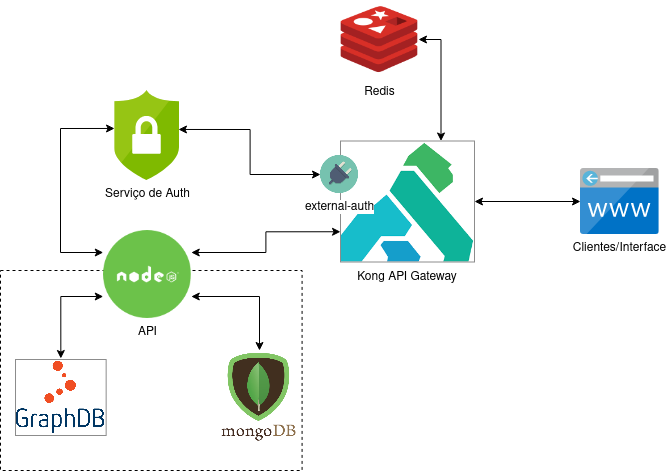
\includegraphics[width=1\textwidth]{img/apiGatewayArchFinal.png}
    \end{center}
    \caption{Arquitetura desenvolvida com \textit{\acrshort{api} Gateway}}\label{fig:apiGatewayArchFinal}
\end{figure}

\section{Resumo}
%TODO
TODO
